\documentclass[notes=show,smaller,handout]{beamer}
%%%%%%%%%%%%%%%%%%%%%%%%%%%%%%%%%%%%%%%%%%%%%%%%%%%%%%%%%%%%%%%%%%%%%%%%%%%%%%%%%%%%%%%%%%%%%%%%%%%%%%%%%%%%%%%%%%%%%%%%%%%%%%%%%%%%%%%%%%%%%%%%%%%%%%%%%%%%%%%%%%%%%%%%%%%%%%%%%%%%%%%%%%%%%%%%%%%%%%%%%%%%%%%%%%%%%%%%%%%%%%%%%%%%%%%%%%%%%%%%%%%%%%%%%%%%
\usepackage{amssymb}
\usepackage{amsmath}
\usepackage{graphicx}
\usepackage{hyperref}
\usepackage{multimedia}
\usepackage{epstopdf}
\usepackage{color}
\usepackage{url}


\setcounter{MaxMatrixCols}{10}
\newtheorem{remark}{Remark}[section]
\newtheorem{proposition}{Proposition}[section]
\newtheorem{interpretation}{Interpretation}[section]
\newtheorem{goal}{Goal}[section]
\newtheorem{statement}{Statement}[section]
\newtheorem{aes}{Aim \& Scope}[section]
\newtheorem{exercise}{Exercise}[section]
\renewcommand{\Pr}{P}

\newcommand{\mbf}[1]{\mathbf{#1}}
\newcommand{\beq}{\begin{equation}}
\newcommand{\eeq}{\end{equation}}
\newcommand{\bea}{\begin{eqnarray}}
\newcommand{\eea}{\end{eqnarray}}
\newcommand{\ba}{\begin{array}}
\newcommand{\ea}{\end{array}}
\newcommand{\bi}{\begin{itemize}}
\newcommand{\ei}{\end{itemize}}
\newcommand{\ben}{\begin{enumerate}}
\newcommand{\een}{\end{enumerate}}
\newcommand{\nn}{\nonumber}

\newenvironment{stepenumerate}{\begin{enumerate}[<+->]}{\end{enumerate}}
\newenvironment{stepitemize}{\begin{itemize}[<+->]}{\end{itemize} }
\newenvironment{stepenumeratewithalert}{\begin{enumerate}[<+-| alert@+>]}{\end{enumerate}}
\newenvironment{stepitemizewithalert}{\begin{itemize}[<+-| alert@+>]}{\end{itemize} }
\usetheme{Madrid}



\begin{document}


\title[S110015]{Probability I}
\subtitle{Lecture 10}
\author[La Vecchia]{Davide La Vecchia (adapted from Prof. Dr. Diego Kuonen)}
\date{Spring Semester 2019}
\maketitle


\begin{frame}
\frametitle{Introduction to simulation}

\color{red} \textbf{Q.} \textit{How can we determine the probability of winning a match in a card game (it does not really matter which game are we talking about, the only relevant point is that we make use of 52 standards playing cards)?} \color{black}

\vspace{1cm}

$\Rightarrow$  Well, actually, the first method that comes to our mind (see Lecture 3) consists in assuming (quite reasonably) that the 
$52!$ permutations of the cards are equally likely. Then, we ``count'' the number of favorable games ... \pause 
Unfortunately, the \textbf{implementation} of this criterion seems quite demanding: $52!$ it is a huge number (even the combinatronics
seems messy!!!)

\vspace{0.4cm}
So, we should, sadly, conclude that  the derivation of the required probability is hardly tractable from a strict mathematical stand point....However, 
we can decide to ``drop '' the rigorous mathematical treatment and invoke an approach which is pretty standard
in the applied science: we make use of an \textbf{experiment} to gain insights and further understanding.


\end{frame}


\begin{frame}
\frametitle{Introduction to simulation}

For instance,  in our case of card game, the \textbf{experiment} consists in playing a (very) large number of games and count the numbers of favorable events (we win).

\vspace{0.4cm}

So, after the execution of $n$ (say) games we will be able to set:
$$
X_i = \left\{\begin{array}{ll}
1& \mbox{ if the $i$-th game is a victory}\\
0 & \mbox{ else}
\end{array}\right.
$$
where the variables $X_i$, for $i=1,...n$ are random variables, each having a Bernoulli distribution such that
$$
E(X_i) = P(\text{win the card game}) = p.
$$

\end{frame}


\begin{frame}
\frametitle{Introduction to simulation}
Now, invoking the WLLN, we have that
$$
\bar{X}_n = \frac{\sum_{i=1}^n X_i}{n} = \frac{\text{\# of favorable games}}{\text{\# of total games played}}
$$
converges, as $n \to \infty$, in probability to $p$, i.e. the probability of winning. \pause \\

\vspace{0.4cm}

In words, we can claim that after a large number of games the proportion
of games that we win can be reasonably applied to get an estimate of $p$. 
\vspace{0.4cm}

\begin{definition} 
The method which determines/estimates the probability ($p$) using experimentation (e.g., performing a long experiment in a computer, as in our example) is called \textbf{simulation}.
\end{definition} 


\end{frame}



\begin{frame}
\frametitle{Simulation procedure}

The remaining issue is that we have typically no
time to play such a big number of games, so we let a computer play. 
%We, typically, have no time to play a large number of card games, so we exploit a computer. 
With this aim

\begin{itemize}
\item we should generate values from a random  variable 
having $U(0,1)$ distribution: these values are called \textit{random numbers}. 

\item Starting from a $U \sim U(0,1)$ distribution, we can in principle simulate any random variable having a CDF, by means of the $F^{-1}$ transformation % (see tutorial, $Y=F^{-1}(U)$).

\end{itemize}

\begin{remark}
In fact, the computer makes use of the so called \textbf{generator of pseudo random numbers}: an algorithm produces a sequence of numbers which are (only) pseudo-
random. Namely, the generator yields a sequence of numbers that, PRACTICALLY, is VERY SIMILAR to a sample drawn form $U(0,1)$. The way in which this algorithm works is behind the scope of this course: let's simply say that you can use the statistical software to achieve the task. 
\end{remark}



\end{frame}



\begin{frame}
\frametitle{Simulation in R}

For instance, a well-know (freely available software) is R:

\begin{center}
\url{https://cran.r-project.org}	
\end{center}


\medskip

and 1 realization of a r.v  $B(10, 0.5)$ can be obtained as:

\medskip

\begin{center} % set.seed(2)
\begin{figure}[ptb]\centering
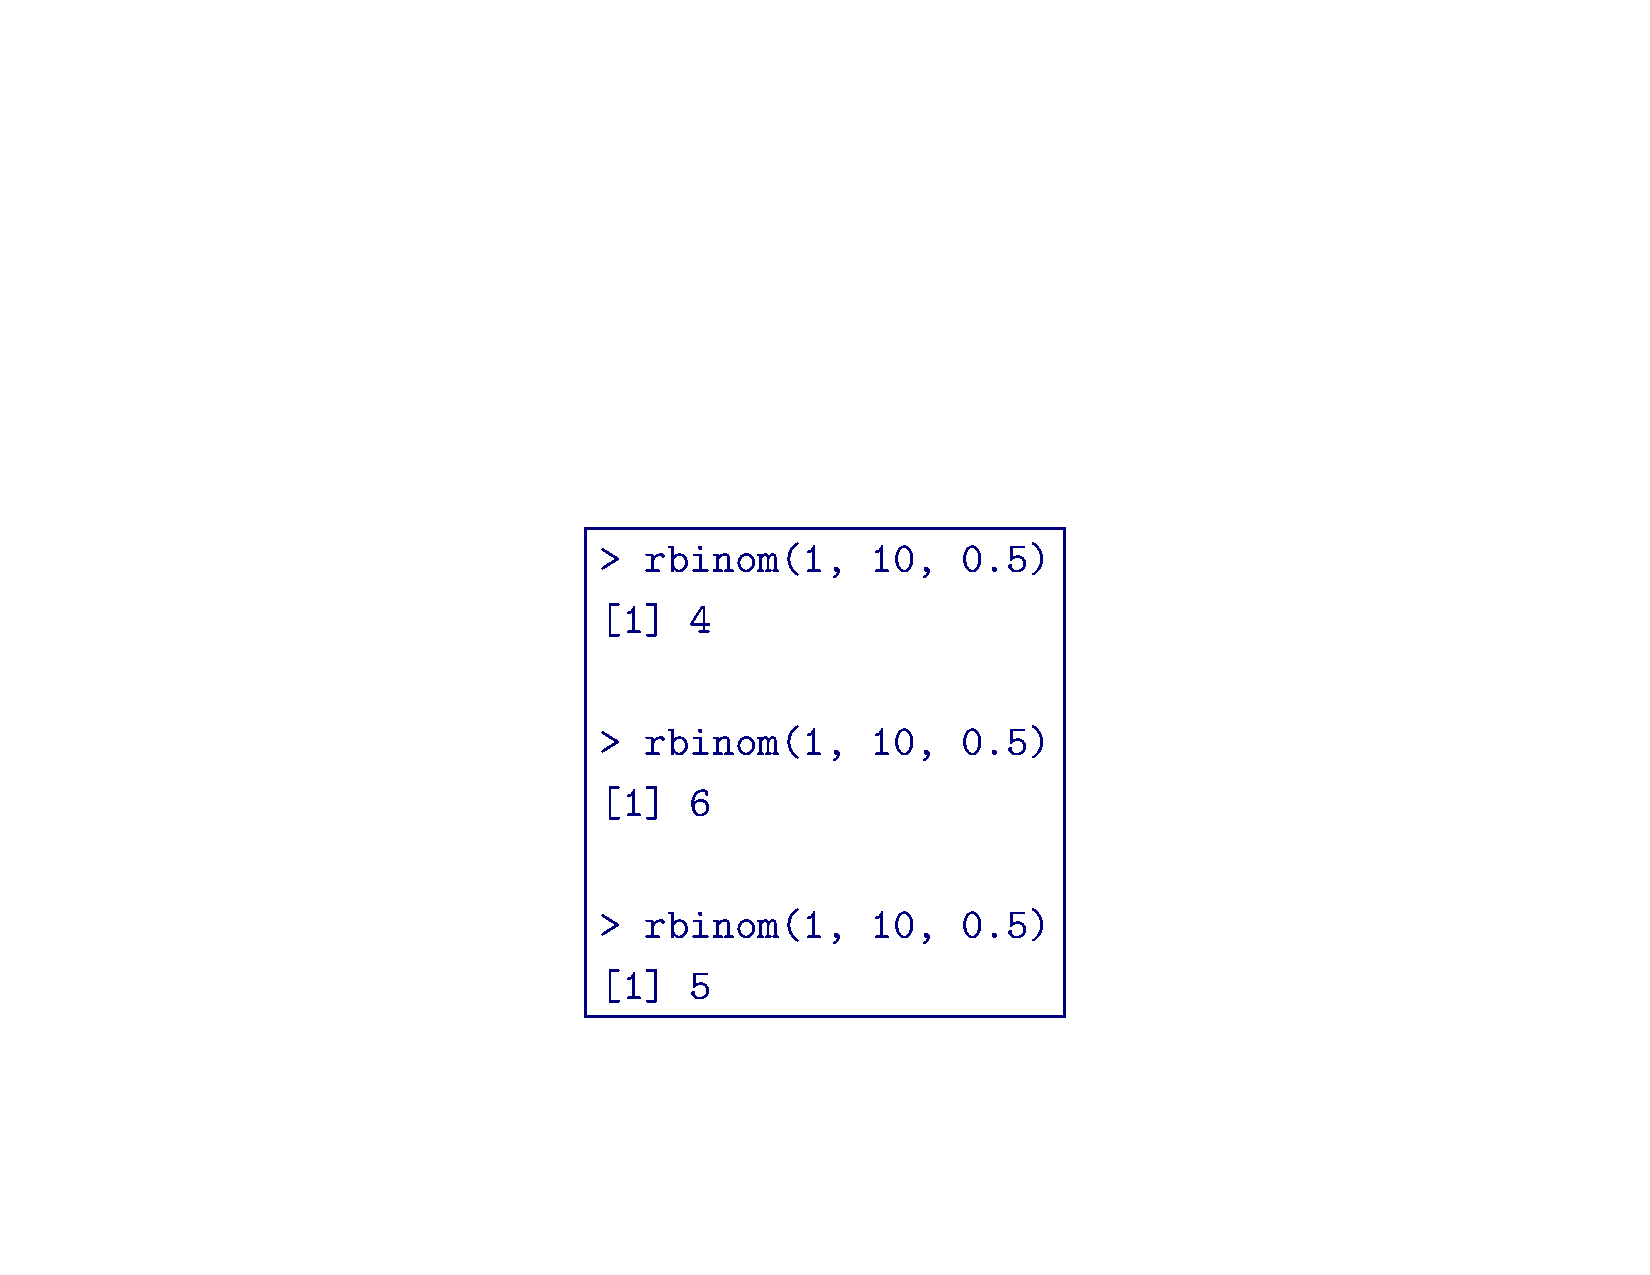
\includegraphics[width=0.35\textwidth,height=0.35\textheight]{sim1.pdf}
\end{figure}

\end{center}
\end{frame}



\begin{frame}
\frametitle{Simulation in R}


and 5 realization of a r.v.'s  $B(10, 0.5)$ can be obtained as:

\medskip

\begin{center} % set.seed(2)
\begin{figure}[ptb]\centering
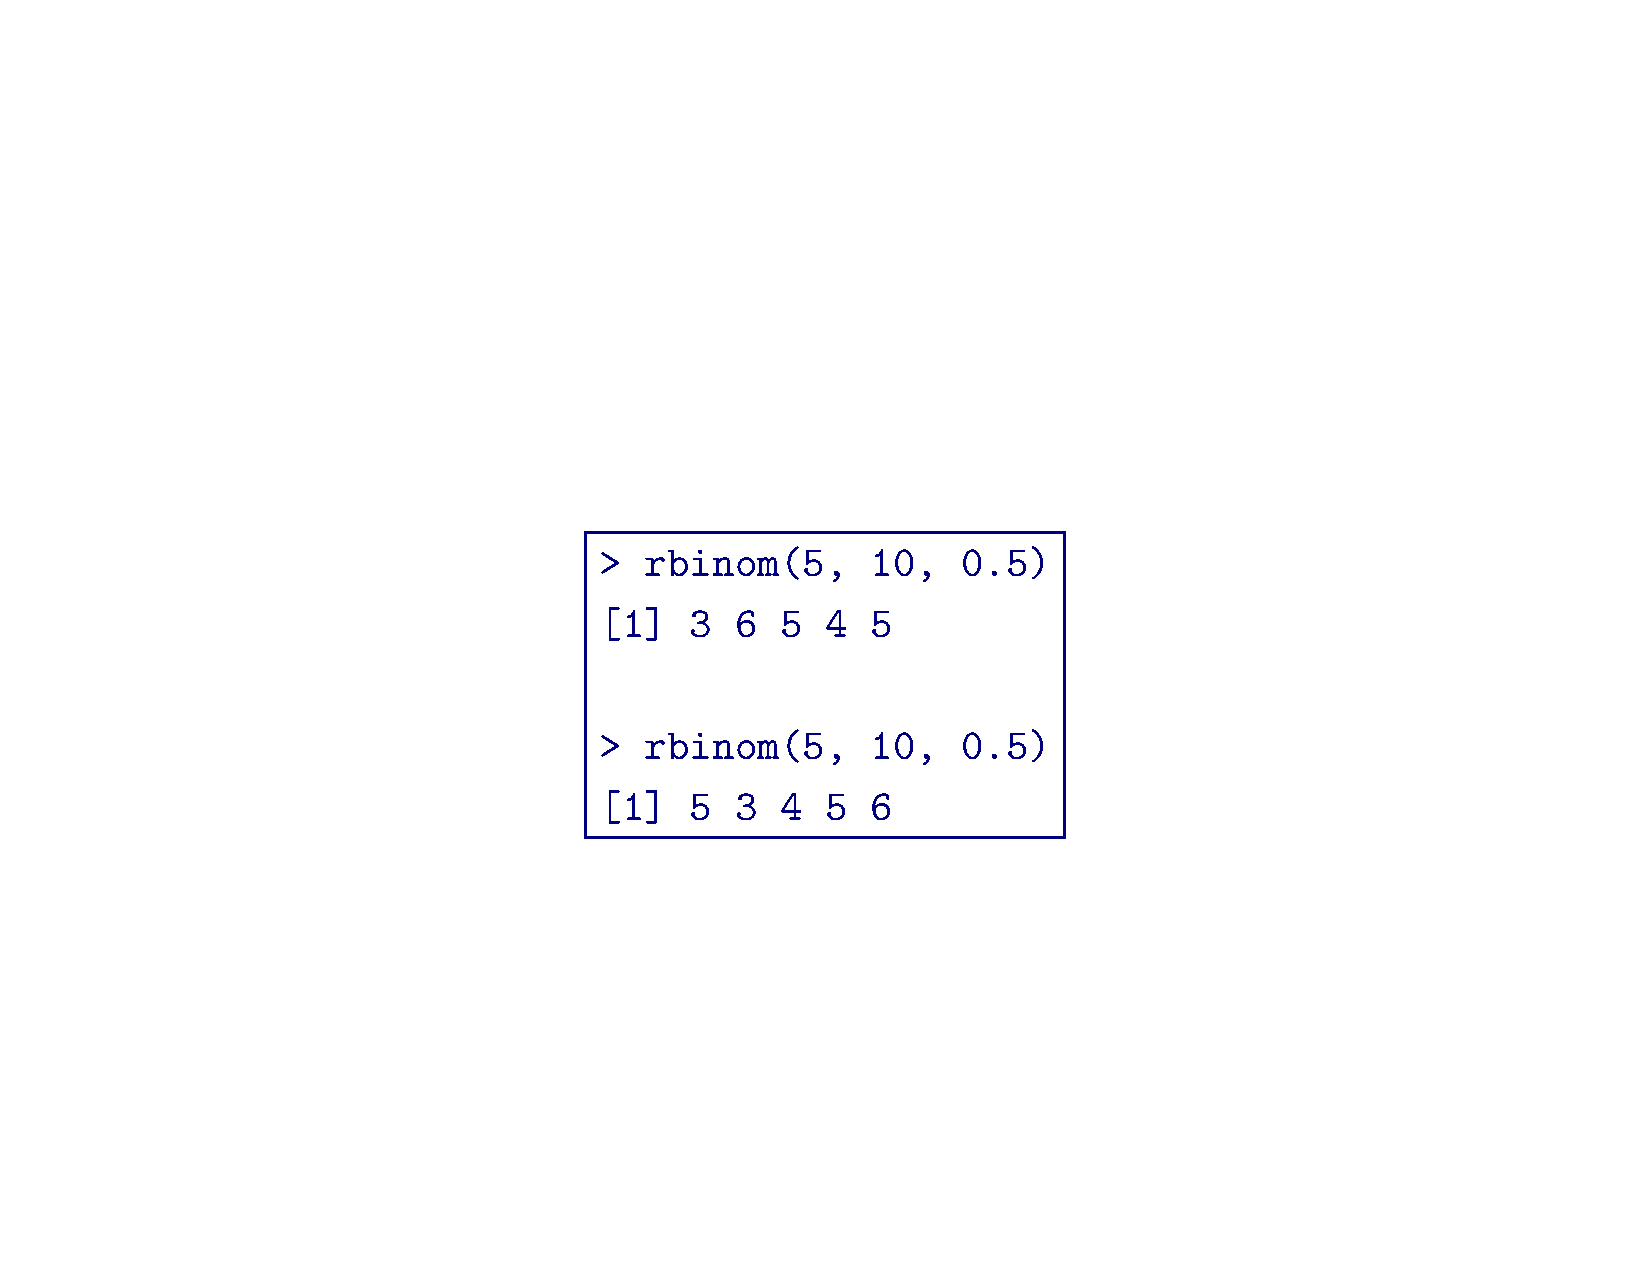
\includegraphics[width=0.35\textwidth,height=0.3\textheight]{sim2.pdf}
\end{figure}

\end{center}
\end{frame}





\begin{frame}
\frametitle{Simulation in R}


and 1 realization of a r.v.'s  $U(0, 1)$ can be obtained as:

\medskip

\begin{center} % set.seed(2)
\begin{figure}[ptb]\centering
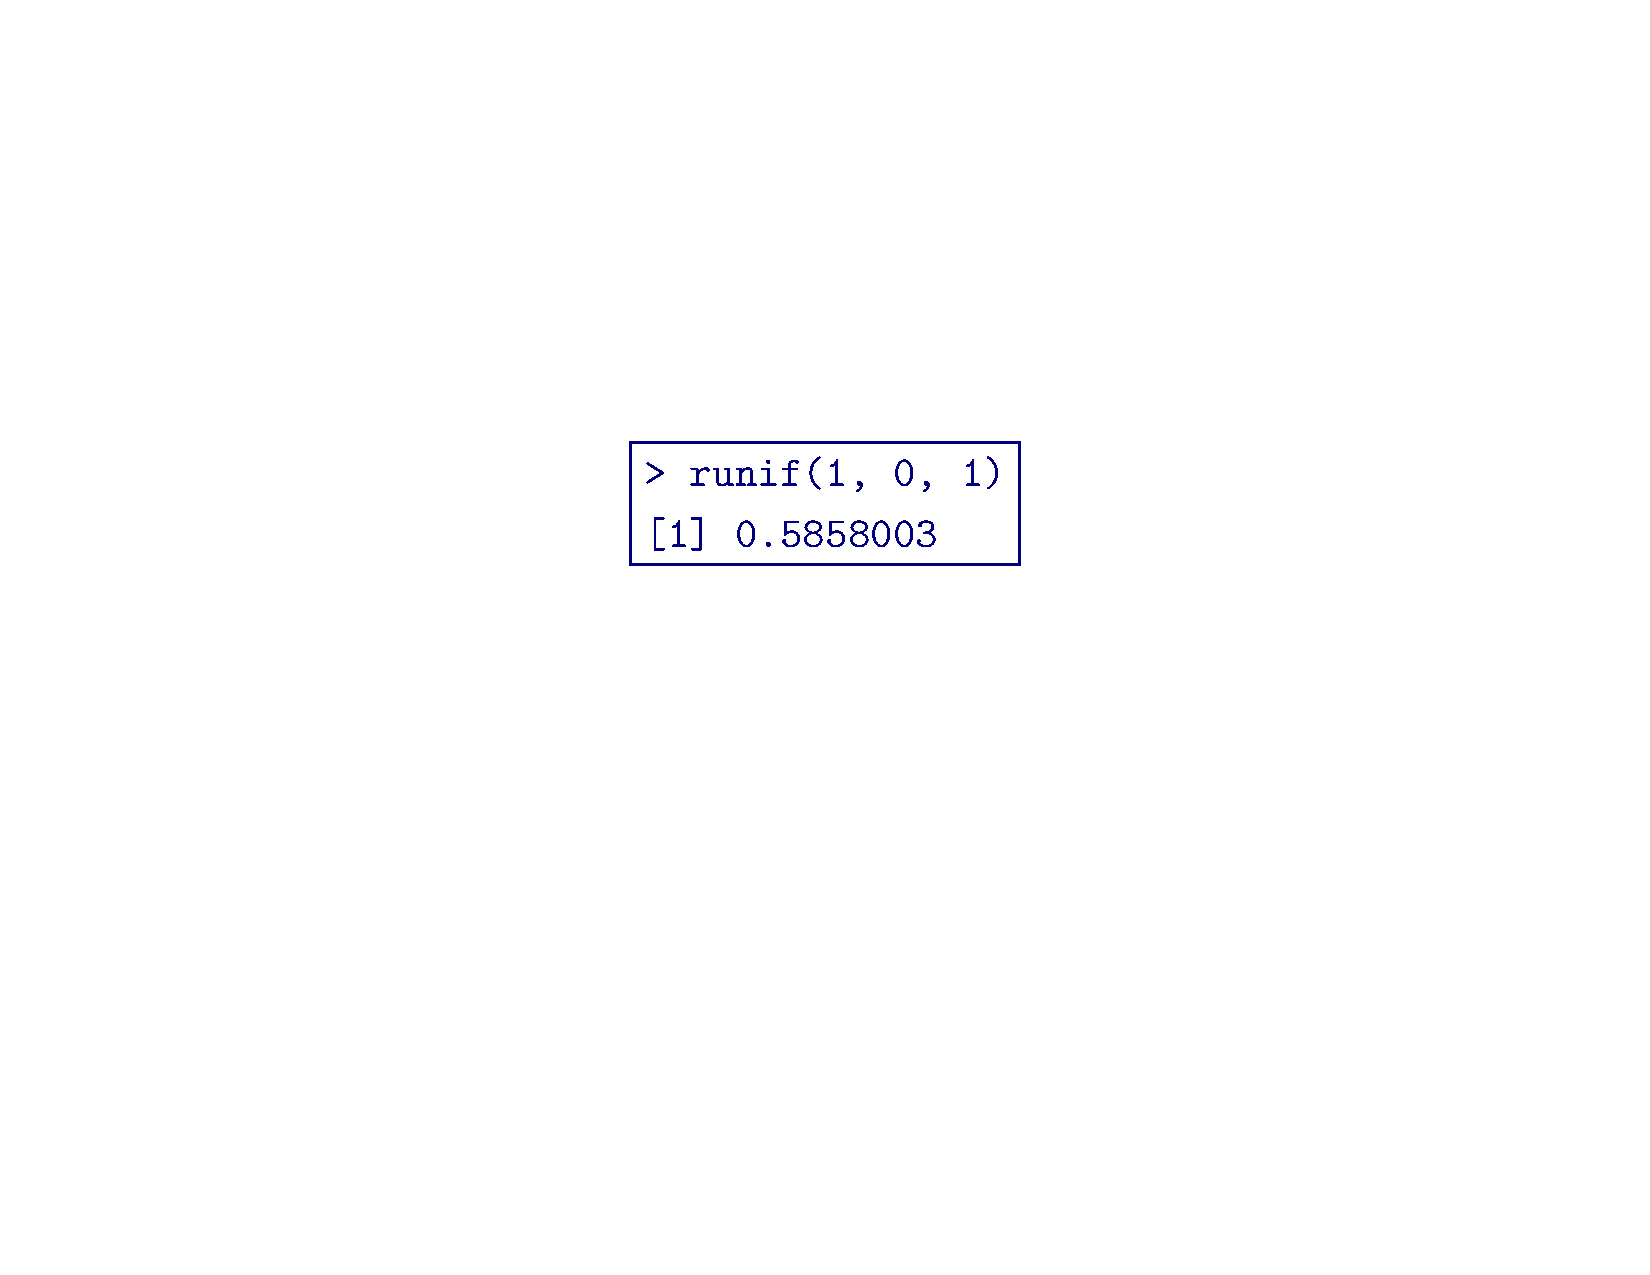
\includegraphics[width=0.25\textwidth,height=0.15\textheight]{sim3.pdf}
\end{figure}
\end{center}

and 5 realization of a r.v.'s  $U(0, 1)$ can be obtained as:

\medskip

\begin{center} % set.seed(2)
\begin{figure}[ptb]\centering
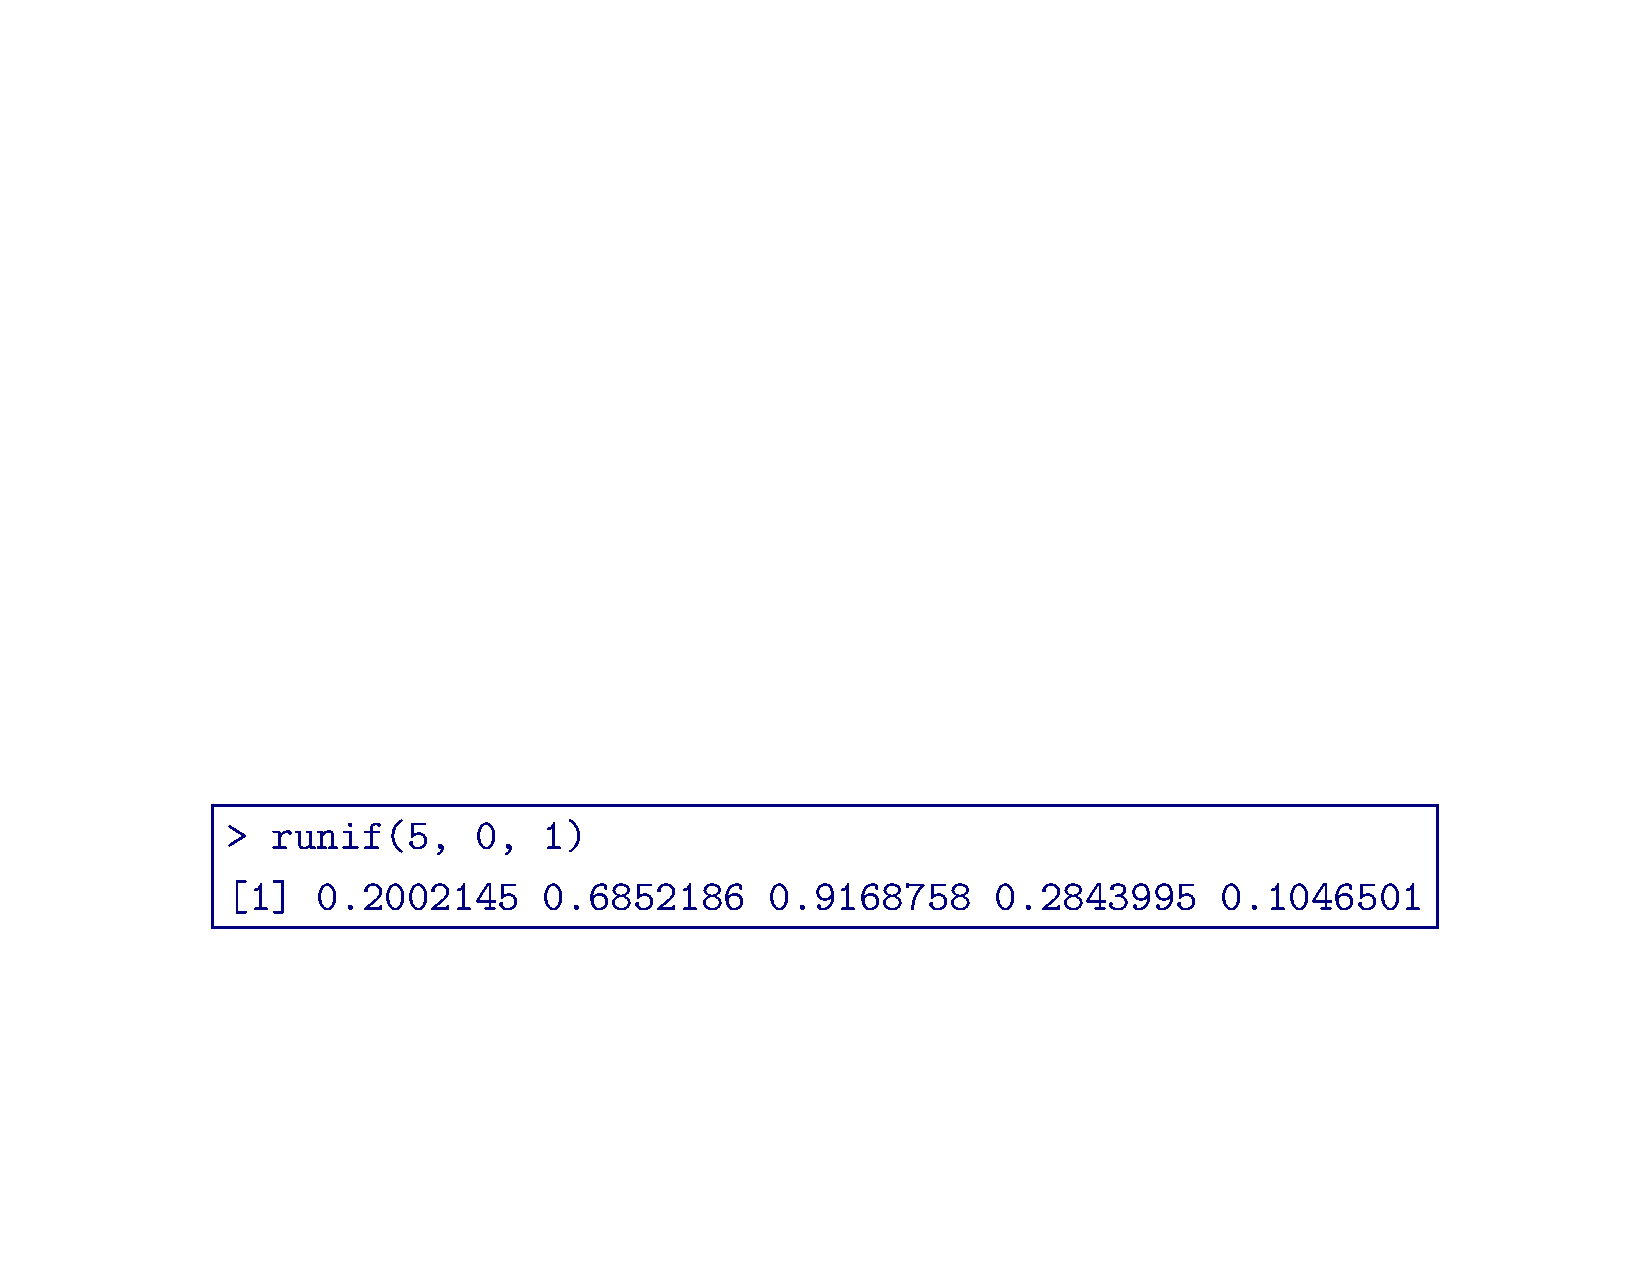
\includegraphics[width=0.75\textwidth,height=0.15\textheight]{sim4.pdf}
\end{figure}
\end{center}
\end{frame}





\begin{frame}
\frametitle{Coin tossing}

A computer cannot toss a coin, 


\begin{center} % set.seed(2)
\begin{figure}[ptb]\centering

\includegraphics[width=0.75\textwidth,height=0.65\textheight]{sim5.pdf}
\end{figure}
\end{center}



but it can generate Bernoulli random numbers....

 

\end{frame}






\begin{frame}
\frametitle{Coin tossing}

...so that we can simulate the outcomes of fair coin $P(H)=P(T)=0.5$

\begin{center} % set.seed(2)
\begin{figure}[ptb]\centering
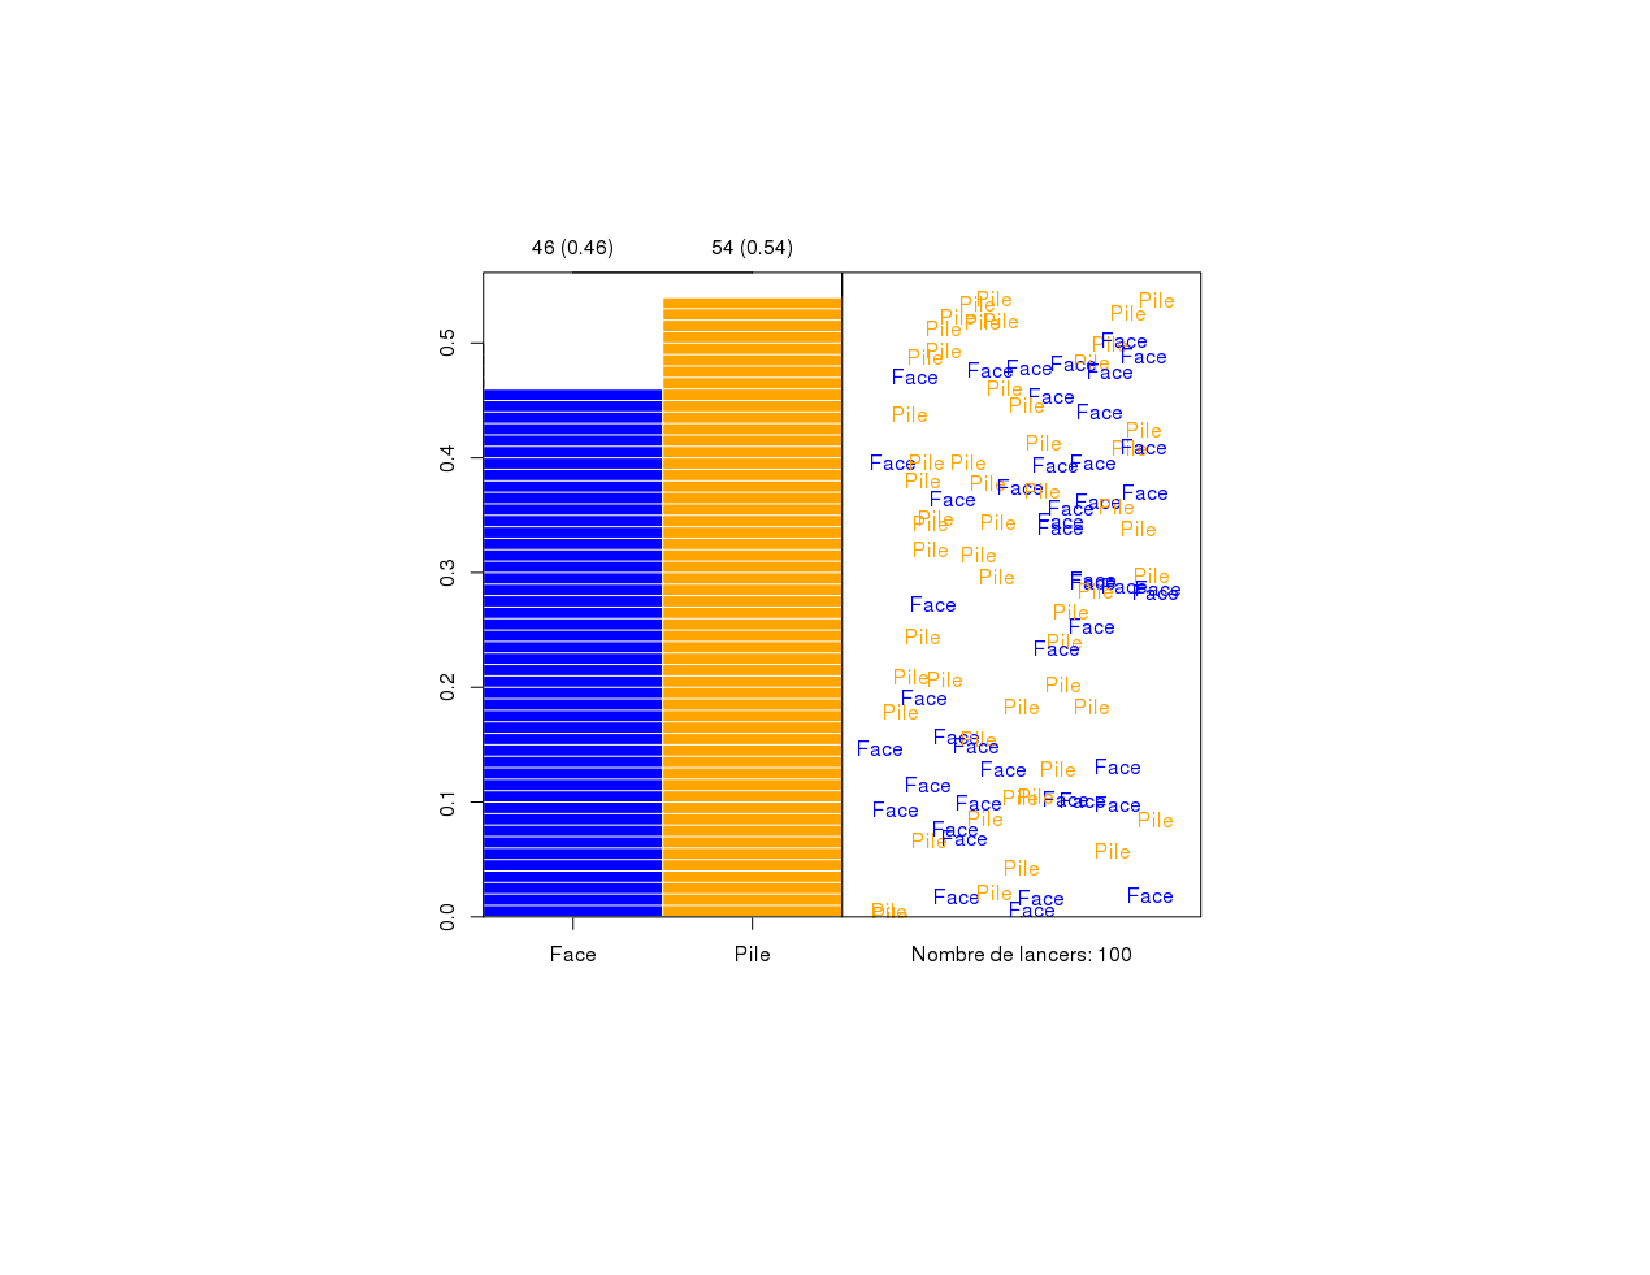
\includegraphics[width=0.5\textwidth,height=0.65\textheight]{sim6.pdf}
\end{figure}
\end{center}



\end{frame}


\begin{frame}
\frametitle{Coin tossing}

...or (exotic case) we can simulate the outcomes of unbalanced coin $P(T)=0.8$

\begin{center} % set.seed(2)
\begin{figure}[ptb]\centering
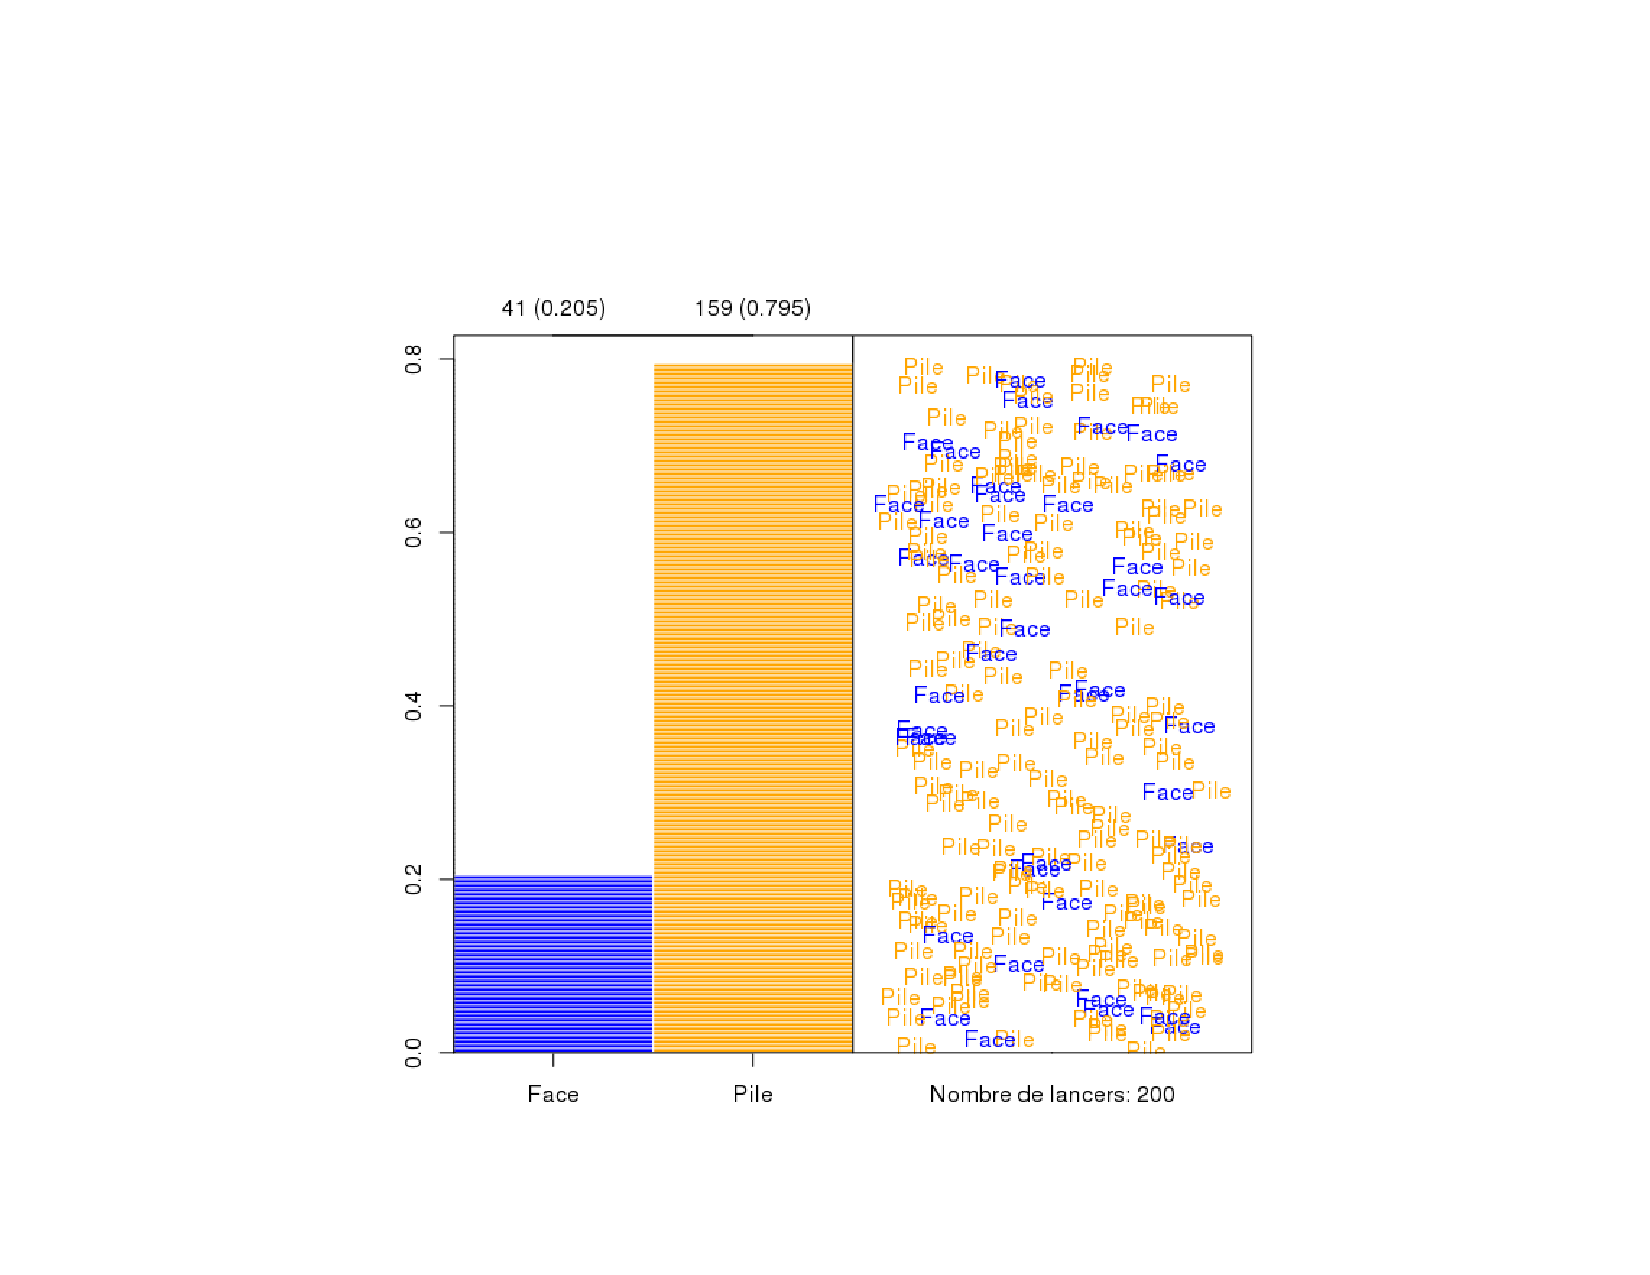
\includegraphics[width=0.55\textwidth,height=0.6\textheight]{sim7.pdf}
\end{figure}
\end{center}



\end{frame}


\begin{frame}
\frametitle{Coin tossing}

...or (even more exotic) we can simulate the outcomes of unbalanced coin $P(H)=P(T)=0.45$ and probability of remaining
 on its edge $0.1$


\begin{center} % set.seed(2)
\begin{figure}[ptb]\centering
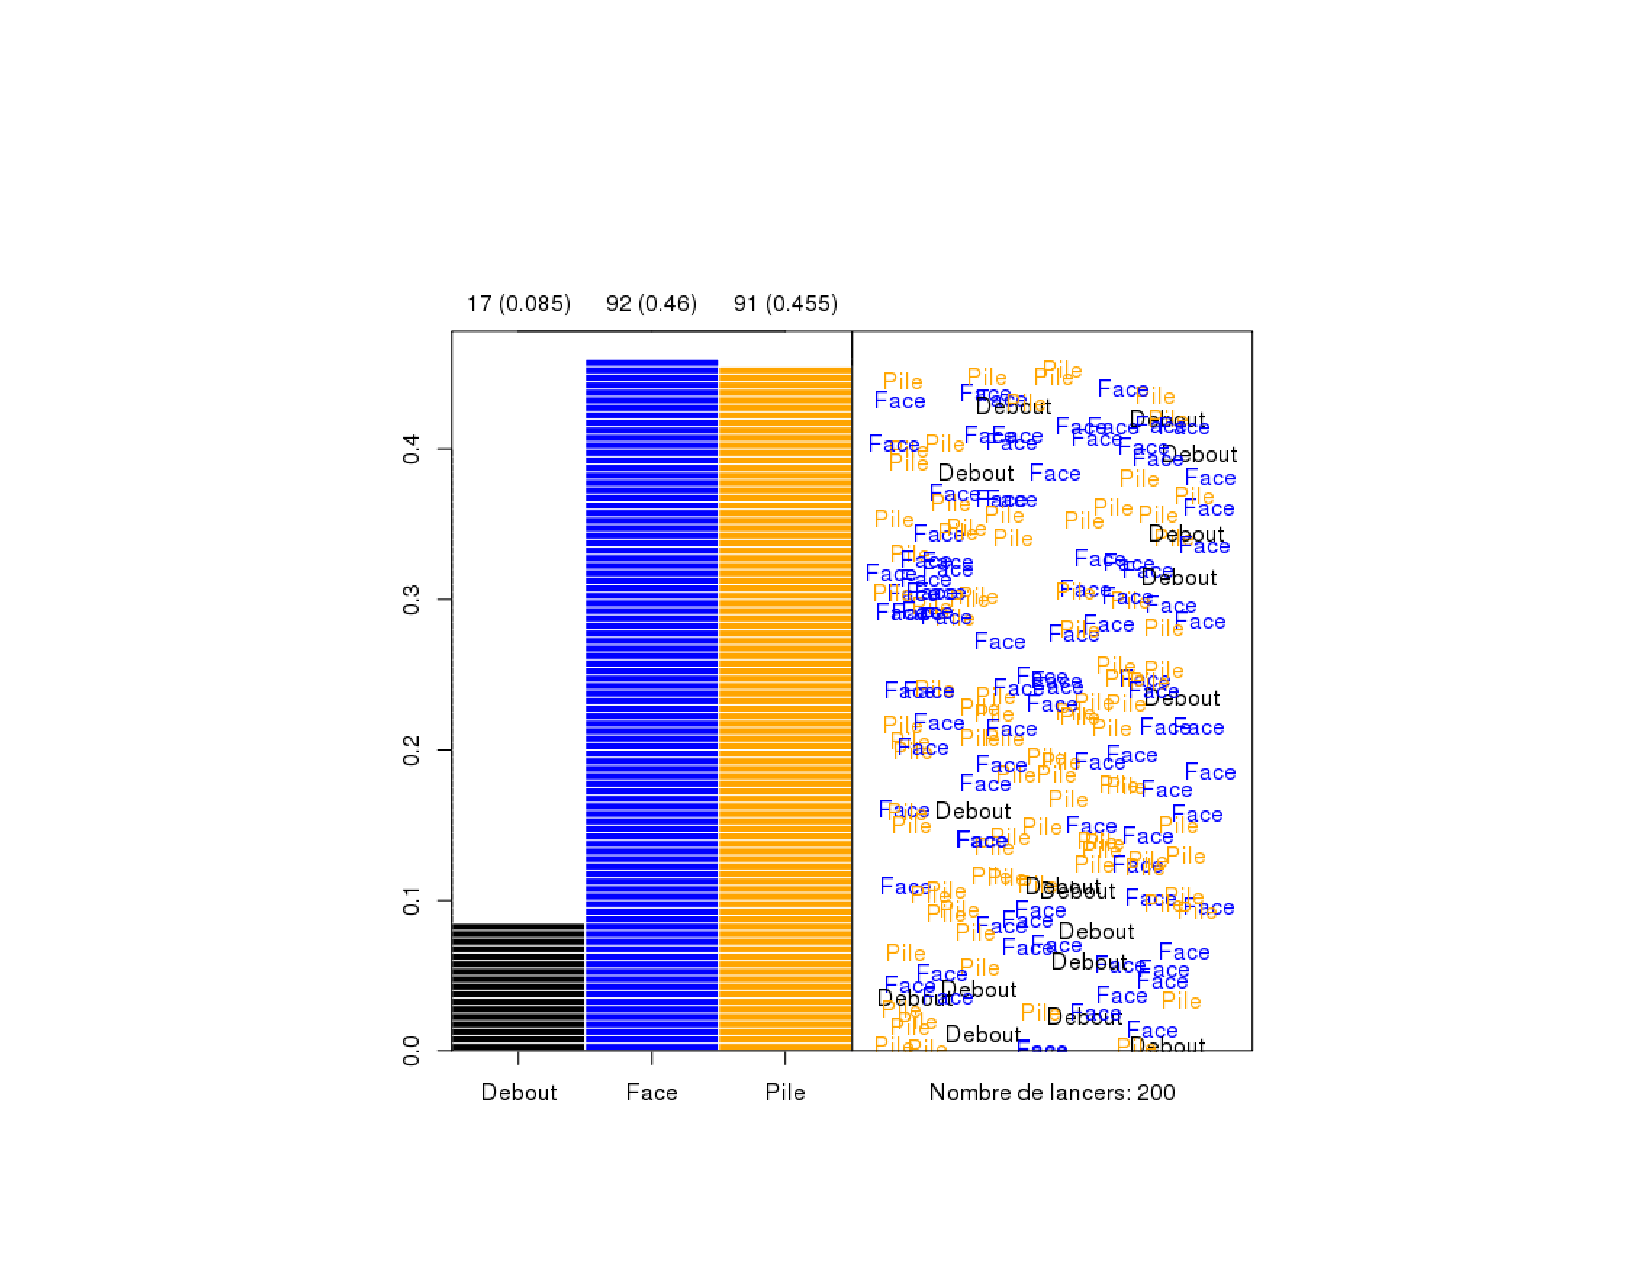
\includegraphics[width=0.55\textwidth,height=0.6\textheight]{sim8.pdf}
\end{figure}
\end{center}



\end{frame}


\begin{frame}
\frametitle{Summarizing}

\begin{remark}
We can make use of the computer power of calculus to shed light on some probabilistic questions.\\ The use of the computer power of calculus and the theory of probability are not mutually exclusive. Rather, I firmly believe that they complement each other: using the computer without any underpinning theoretical development is pointless, while the development of probability theory can strongly benefit from the use of computer power of calculus. 
\end{remark}



\end{frame}



\end{document}

